\documentclass{scrartcl}

\usepackage{graphicx}
\usepackage[utf8]{inputenc}
\usepackage[T1]{fontenc}
\usepackage{lmodern}
\usepackage[english]{babel}
\usepackage{amsmath}
\usepackage{amsthm}
\usepackage{mathtools}
\usepackage{amssymb}
\usepackage{listings}
\usepackage{xparse}
\usepackage{geometry}
\usepackage{enumerate}
\usepackage{tikz}
\usepackage{hyperref}
\usepackage[style=english]{csquotes}
\usepackage[language=english, backend=biber, style=alphabetic, sorting=nyt]{biblatex}

\hypersetup{
    colorlinks,
    linkcolor={red!50!black},
    citecolor={blue!50!black},
    urlcolor={blue!80!black}
}

\usetikzlibrary{babel, positioning, shapes.geometric, arrows, arrows.meta}
\addbibresource{bibliography.bib}

\title{Definition of Schemes}
\author{Simon Pohmann}

\newcommand{\N}{\mathbb{N}}
\newcommand{\Z}{\mathbb{Z}}
\newcommand{\F}{\mathbb{F}}
\newcommand{\I}{\mathbb{I}}
\newcommand{\V}{\mathbb{V}}
\newcommand{\C}{\mathbb{C}}
\newcommand{\p}{\mathfrak{p}}
\newcommand{\Set}{\mathrm{\textbf{Set}}}
\newcommand{\Aff}{\mathrm{\textbf{Aff}}}
\newcommand{\Sch}{\mathrm{\textbf{Sch}}}
\newcommand{\Ring}{\mathrm{\textbf{Ring}}}
\newcommand{\Proj}{\mathbb{P}}
\newcommand{\Half}{\mathcal{H}}
\newcommand{\Top}{\mathrm{Top}}
\newcommand{\SL}{\mathrm{SL}}
\newcommand{\End}{\mathrm{End}}
\newcommand{\Spec}{\mathrm{Spec}}
\newcommand{\Quot}{\mathrm{Quot}}
\renewcommand{\O}{\mathcal{O}}
\DeclareMathOperator*{\colim}{colim}

\newcommand\restr[2]{{
    \left.\kern-\nulldelimiterspace
    #1
    \vphantom{\big|}
    \right|_{#2}
}}

\newtheorem{prop}{Proposition}[section]
\newtheorem{theorem}[prop]{Theorem}
\newtheorem{lemma}[prop]{Lemma}
\newtheorem{corollary}[prop]{Corollary}

\theoremstyle{definition}
\newtheorem{problem}[prop]{Problem}
\newtheorem{alg}[prop]{Algorithm}
\newtheorem{definition}[prop]{Definition}
\newtheorem{example}[prop]{Example}
\newtheorem{remark}[prop]{Remark}

\begin{document}
\maketitle
\tableofcontents

\section{Category-theoretical stuff}
Let $\mathcal{C}$ be a small sub-category of $\Set$ that has small limits and colimits, and let $X$ be a topological space.
\begin{definition}
    A \emph{sheaf} on $X$ is a functor
    \begin{equation*}
        F: \Top(X)^{\mathrm{op}} \to \mathcal{C}
    \end{equation*}
    that satisfies a local-to-global condition, i.e. for $(U_i)_i$ open and $s_i \in F(U_i)$ such that
    \begin{equation*}
        \restr{s_i}{U_i \cap U_j} = \restr{s_j}{U_i \cap U_j}
    \end{equation*}
    there exists a unique $s \in F(\bigcup_i U_i)$ such that
    \begin{equation*}
        \restr{s}{U_i} = s_i
    \end{equation*}
    Here we write $\restr{s}{V}$ for the image of $s \in F(U)$ under the map $F(U) \to F(V)$ (which we get from the inclusion morphism $V \subseteq U$ in $\Top(X)$).
\end{definition}
\begin{definition}
    Let $F$ be a sheaf on $X$. Then the \emph{stalk} of $F$ at some $x \in X$ is the colimit
    \begin{equation*}
        F_x := \colim_{U \ni x \ \text{open}} F(U)
    \end{equation*}
\end{definition}
\begin{definition}
    Let $B$ be a basis of $X$.
    A $B$-sheaf is a functor
    \begin{equation*}
        F: \underbrace{\restr{\Top(X)}{B}^{\mathrm{op}}}_{\mathclap{\text{The subcategory of $\Top(X)$ containing only the objects from $B$}}} \to \mathcal{C}
    \end{equation*}
    that satisfies a local-to-global condition, i.e. for $(U_i)_i$ in $B$ and $s_i \in F(U_i)$ such that
    \begin{equation*}
        \forall x \in U_i \cap U_j \ \underbrace{\exists x \in V \subseteq U_i \cap U_j}_{\mathclap{\text{Since $B$ is a basis, there is always at least one such $V$}}}: \ \restr{s_i}{V} = \restr{s_j}{V} \quad \text{and} \quad U := \bigcup_i U_i \in B
    \end{equation*}
    there exists a unique $s \in F(U)$ such that
    \begin{equation*}
        \restr{s}{U_i} = s_i
    \end{equation*}
\end{definition}
\begin{theorem}
    \label{prop:extend_b_sheaves}
    Let $F$ be a $B$-sheaf for some basis $B$ of $X$.
    Then there exists a unique (up to unique isomorphism) sheaf $\tilde{F}$ on $X$ that extends $F$.
\end{theorem}
\begin{proof}
    First, we show Existence. For an open $U$ in $X$, define
    \begin{equation*}
        \tilde{F}(U) := \lim_{V \subseteq U, \ V \in B} F(V)
    \end{equation*}
    For an inclusion $U_1 \subseteq U_2$ and $s \in \tilde{F}(U_2)$, define then $\tilde{F}(U_1 \subseteq U_2)$ as the unique map such that
    \begin{equation*}
        \tilde{F}(U_2) \overset{\tilde{F}(U_1 \subseteq U_2)}{\to} \tilde{F}(U_1) \to F(V) \quad \text{is} \quad \tilde{F}(U_1) \to F(V)
    \end{equation*}
    for all $V \subseteq U_1, \ V \in B$.
    
    Now note that for $U_1 \subseteq U_2 \subseteq U_3$ we also have a map
    \begin{equation*}
        \tilde{F}(U_3) \to \tilde{F}(U_2) \to \tilde{F}(U_1)
    \end{equation*}
    that is compatible with the maps $F(V_1 \subseteq V_2)$ for $V_1 \subseteq V_2, \ V_1, V_2 \in B$, and so by uniqueness above, we see
    \begin{equation*}
        \tilde{F}(U_1 \subseteq U_3) = \tilde{F}(U_1 \subseteq U_2) \circ \tilde{F}(U_2 \subseteq U_3)
    \end{equation*}
    Furthermore, clearly $\tilde{F}(\mathrm{id}_U) = \mathrm{id}_{\tilde{F}(U)}$, so $\tilde{F}$ is a presheaf.
    Note that $\tilde{F}(V) \cong F(V)$ for all $V \in B$ and similar for morphisms, so indeed $\tilde{F}$ extends $F$.

    Now we show the local-to-global condition.
    Assume we have $(U_i)_i$ open in $X$ and $s_i \in \tilde{F}(U_i)$ such that
    \begin{equation*}
        \restr{s_i}{U_i \cap U_j} = \restr{s_j}{U_i \cap U_j}
    \end{equation*}
    Let $U = \bigcup_i U_i$. 
    By the local-to-global condition of $F$, for each $ V \subseteq U, \ V \in B$ there exists a unique $s_V \in \tilde{F}(V) = F(V)$ with
    \begin{equation*}
        \restr{s_V}{V_i} = \restr{s_i}{V_i} \quad \text{for all $V_i \subseteq U_i \cap V, \ V_i \in B$}
    \end{equation*}
    Since
    \begin{equation*}
        \lim_{V \subseteq U, \ V \in B} F(V) \cong \bigl\{ (a_V)_V \in \prod_V F(V) \bigm| F(V_1 \subseteq V_2)(a_{V_2}) = a_{V_1} \bigr\}
    \end{equation*}
    we see that these $s_V$ lift to one (necessarily unique) $s \in \tilde{F}(U)$.

    For Uniqueness, assume we have two such sheaves, say $G$ and $H$.
    Now note that for all open $U$ in $X$ with $V_i \in B$, we have
    \begin{equation*}
        G(U) \cong \bigl\{ (a_V)_V \in \prod_{V \subseteq U, \ V \in B} F(V) \bigm| F(V_1 \subseteq V_2)(a_{V_2}) = a_{V_1} \bigr\}
    \end{equation*}
    where $\supseteq$ follows from general structure and $\subseteq$ from the local-to-global property.
    The same holds for $H$, so $G \cong H$.
\end{proof}

\section{Schemes}
\begin{definition}
    A \emph{locally ringed space} is a topological space $X$ with a sheaf of rings $\O_X$ on $X$ such that all stalks $\O_{X, x}$ are local rings.
\end{definition}
\begin{definition}
    Let $R$ be a ring (commutative, unital).
    Then let $\O_{\Spec R}$ be the sheaf on $\Spec R$ that results from extending the B-sheaf
    \begin{equation*}
        \O_{\Spec R}(D_f) := R_f, \quad f \in R
    \end{equation*}
    to a sheaf as in Theorem~\ref{prop:extend_b_sheaves}.
    Here the sets
    \begin{equation*}
        D_f = \{ \mathfrak{p} \leq R \ | \ f \notin \mathfrak{p} \} \subseteq \Spec R
    \end{equation*}
    are the basic open sets and form a basis of $\Spec R$.
\end{definition}
\begin{definition}
    A morphism between locally ringed spaces $(X, \O_X)$ and $(Y, \O_Y)$ is a continuous map $f: X \to Y$ together with a natural transformation $\eta: \O_Y \Rightarrow f_*\O_X$ that satisfies
    \begin{equation*}
        \eta_y: (f_*\O_X)_y \cong \O_{X, f(y)} \to \O_{Y, y} \quad \text{maps} \quad \eta_y(\mathfrak{m}) \subseteq \mathfrak{m}
    \end{equation*}
    for all $y \in Y$.

    Here
    \begin{equation*}
        f_*: \mathrm{Sh}(X) \to \mathrm{Sh}(Y), \quad F \mapsto (U \mapsto F(f^{-1}(U)))
    \end{equation*}
    is the pullback of $f$.
\end{definition}
\begin{definition}
    A locally ringed space $(X, \O_X)$ is an \emph{affine scheme}, if there exists a ring $R$ such that $(X, \O_X) \cong (\Spec R, \O_{\Spec R})$.
\end{definition}
\begin{definition}
    A locally ringed space $(X, \O_X)$ is a \emph{scheme}, if there exists a covering $X = \bigcup_i U_i$ with open $U_i \subseteq X$ such that each $(U_i, \restr{\O_X}{U_i})$ is an affine scheme.
\end{definition}
\begin{definition}
    A \emph{morphism} of locally ringed spaces $(X, \O_X) \to (Y, \O_Y)$ is a continuous map $f: X \to Y$ and a morphism of sheaves
    \begin{equation*}
        \phi: \O_Y \to f_*\O_X
    \end{equation*}
    such that each
    \begin{equation*}
        \phi_x: \O_{Y, f(x)} \to \O_{X, x}
    \end{equation*}
    is a homomorphism of local rings.
    Here $f_*\O_X$ is the sheaf $(f_*\O_X)(U) := \O_X(f^{-1}(U))$.
\end{definition}
\begin{definition}
    Denote the category of schemes by $\Sch$ and the subcategory of affine schemes by $\Aff$
\end{definition}
\begin{definition}
    Let $\phi: R \to S$ be a ring homomorphism.
    Then this induces a morphism of affine schemes
    \begin{equation*}
        \Spec\phi: \Spec S \to \Spec R
    \end{equation*}
    given by
    \begin{equation*}
        \Spec\phi: \p \mapsto \phi^{-1}(\p)
    \end{equation*}
    and on basic open sets $D_g, \ g \in R$ by
    \begin{equation*}
        (\Spec\phi)_{D_g}: \O_{\Spec R}(D_g) \to \O_{\Spec S}(D_{\phi(g)}), \quad \frac x {g^k} \to \frac {\phi(x)} {\phi(g)^k}
    \end{equation*}
\end{definition}
\begin{prop}
    The functor
    \begin{equation*}
        \Spec: \Ring^{\mathrm{op}} \to \Aff
    \end{equation*}
    is an equivalence of categories.
\end{prop}
\begin{prop}
    Let $(X, \O_X)$ be a scheme. Then $X$ is T0.
\end{prop}
\begin{proof}
    Assume not, i.e. there are two points $x, y \in X$ such that every open neighborhood of $x$ contains $y$ and vice versa.
    As $(X, \O_X)$ has a cover by affine opens, consider an affine open $U$ containing $x, y$.
    Then $(U, \restr{\O_X}{U})$ is isomorphic to $\Spec R$ for some ring $R$.
    However, $\Spec R$ is T0, a contradiction. 
\end{proof}

\section{Coproduct (gluing) in $\Sch$}

\begin{prop}
    For affine schemes $\Spec R_1$ and $\Spec R_2$ have that the coproduct in $\Sch$ is
    \begin{equation*}
        \Spec R_1 \sqcup \Spec R_2 = \Spec(R_1 \times R_2)
    \end{equation*}
\end{prop}
\begin{proof}
    Observe that
    \begin{equation*}
        \Spec(R_1 \times R_2) = \underbrace{\{ \p \times R_2 \ | \ \p \in \Spec R_1 \}}_{=: V_1} \cup \underbrace{\{ R_1 \times \p \ | \ \p \in \Spec R_2 \}}_{=: V_2}
    \end{equation*}
    First of all, the projection maps $\pi_i: R_1 \times R_2 \to R_i$ give rise to morphisms
    \begin{equation*}
        \phi_i: \Spec R_i \to \Spec(R_1 \times R_2)
    \end{equation*}
    So we have to show that this cocone is universal.

    Let $(W, \O_W)$ be a scheme with morphisms
    \begin{equation*}
        \psi_i: \Spec R_i \to (W, \O_W)
    \end{equation*}
    Define
    \begin{equation*}
        f: \Spec(R_1 \times R_2) \to W, \quad \begin{matrix*}
            \p \times R_2 &\mapsto\ \psi_1(\p) \\
            R_1 \times \p &\mapsto\ \psi_2(\p)
        \end{matrix*}
    \end{equation*}
    This is well-defined, as $\psi_i(R_i)$ is a point such that $\psi_i(\Spec R_i)$ is contained in every open neighborhood of it.
    Hence $\psi_1(R_1)$ and $\psi_2(R_2)$ cannot be separated by open sets, and thus must be equal as $W$ is T0.

    Furthermore, for any open $U \subseteq W$ note that
    \begin{equation*}
        f^{-1}(U) = \{ \p \times R_2 \ | \ \p \in \psi_1^{-1}(U) \} \cup \{ R_1 \times \p \ | \ \p \in \psi_2^{-1}(U) \}
    \end{equation*}
    is a union of open sets, hence open.
    So $f$ is continuous.

    Now note that
    \begin{equation*}
        (V_i, \restr{\O_{\Spec(R_1 \times R_2)}}{V_i}) \cong \Spec R_i
    \end{equation*}
    where the isomorphisms are natural in $V_i$.
    So $s \in \O_W(U)$ yields via $\O_W(U) \to \O_{\Spec R_i}(\psi^{-1}(U)) \cong \O_{\Spec(R_1 \times R_2)}(f^{-1}(U) \cap V_i)$ elements
    \begin{equation*}
        s'_1 \in \O_{\Spec(R_1 \times R_2)}(f^{-1}(U) \cap V_1), \quad s'_2 \in \O_{\Spec(R_1 \times R_2)}(f^{-1}(U) \cap V_2)
    \end{equation*}
    These glue together to some $s' \in \O_{\Spec(R_1 \times R_2)}(f^{-1}(U))$.
    Hence define a morphism of sheaves
    \begin{equation*}
        \eta: \O_W \to f_*\O_{\Spec(R_1 \times R_2)}, \quad \eta_U(s) := s'
    \end{equation*}
    as it is clearly compatible with restriction maps.

    Now, by construction, have that for $\p \in \Spec R_i$
    \begin{equation*}
        (f \circ \phi_i)(\p) = f(\pi_i^{-1}(\p)) = \psi_i(\p)
    \end{equation*}
    and
    \begin{equation*}
        \phi_i \circ \eta = \psi_i
    \end{equation*}
    The latter is true, as the isomorphism in
    \begin{equation*}
        \O_W(U) \to \O_{\Spec R_i}(\psi_i^{-1}(U)) \cong \O_{\Spec(R_1 \times R_2)}(f^{-1}(U) \cap V_i)
    \end{equation*}
    in the direction $\leftarrow$ on basic open sets is given by the extension of the projection map $\pi_i: (R_1 \times R_2)_g \to (R_i)_{\pi_i(g)}$ and hence is $\phi_i$.

    The uniqueness of the morphism $(f, \eta)$ is clear.
\end{proof}
\begin{prop}
    Let $(U_i)_i$ be a family of schemes with open subschemes $U_{ij} \subseteq U_i$ and isomorphisms $\phi_{ij}: U_{ij} \to U_{ji}$.
    If
    \begin{itemize}
        \item $U_{ii} = U_i$ and $\phi_{ii} = \mathrm{id}$
        \item $\phi_{ij}(U_{ij} \cap U_{ik}) \subseteq U_{ji} \cap U_{jk}$
        \item $\restr{\phi_{ik}}{U_{ij} \cap U_{ik}} = \phi_{jk} \circ \restr{\phi_{ij}}{U_{ij} \cap U_{ik}}$
    \end{itemize}
    then there is a scheme $X$ (unique up to unique isomorphism) with an open cover $X = \bigcup X_i$ and isomorphisms of schemes $\psi_i: U_i \to X_i$ such that
    \begin{equation*}
        \psi_j \circ \phi_{ij} = \restr{\psi_i}{U_{ij}}
    \end{equation*}
\end{prop}
\begin{remark}
    The above easily shows that coproducts exist in $\Sch$ (just take $U_i$ to be the empty scheme $(\emptyset, \emptyset \mapsto \{0\})$).
    However, $\Sch$ is not cocomplete\footnote{\href{https://mathoverflow.net/questions/9961/colimits-of-schemes}{https://mathoverflow.net/questions/9961/colimits-of-schemes}}, so coequalizers do not exist in general.
\end{remark}

\section{Products in $\Sch$}

\begin{prop}
    Let $f: X \to Z$ and $g: Y \to Z$ be schemes over a scheme $Z$.
    The fiber product (or pullback) $X \times_Z Y$ is defined as the limit of
    \begin{equation*}
        X \overset{f}{\rightarrow} Z \overset{g}{\leftarrow} Y
    \end{equation*}
    (Finite) fiber products exist in $\Sch$.
\end{prop}
\begin{proof}
    We show that binary fiber products exist.
    Let $f: X \to Z, \ g: Y \to Z$ be as above.

    \paragraph{Step 1: $X, Y, Z$ affine} Assume $X = \Spec R, \ Y = \Spec S, \ Z = \Spec T$ and $f, g$ are induced by ring homomorphisms
    \begin{equation*}
        f^\#: T \to R, \quad g^\#: T \to S
    \end{equation*}
    We claim that $\Spec(R \otimes_T S)$ with 
    \begin{equation*}
        (\cdot \otimes 1)^\#: \Spec(R \otimes_T S) \to \Spec R, \quad (1 \otimes \cdot)^\#: \Spec(R \otimes_T S) \to \Spec S
    \end{equation*}
    works.
    For this, it suffices to show that $R \otimes_T S$ is the pushout (i.e. co-fiber product) of $R, S$ considered as $T$-algebras.
    This follows easily from the universal property of the tensor product.
    \paragraph{Step 2: $Y, Z$ affine} Assume $Y = \Spec S, \ Z = \Spec T$.
    Let $X = \bigcup X_i$ be a cover of $X$ by affine opens.
    We want to glue all $X_i \times_Z Y$.

    Note that $U_i := X_i \times_Z Y$ comes with a map $\pi_i: U_i \to X_i$.
    Now we can consider the open subscheme
    \begin{equation*}
        U_{ij} := \Bigl( \pi_i^{-1}(X_i \cap X_j), \ \restr{\O_{X}}{\pi_i^{-1}(X_i \cap X_j)} \Bigr)
    \end{equation*}
    Claim: $U_{ij}$ is the fiber product $(X_i \cap X_j) \times_Z Y$.
    Clearly $U_{ij}$ has maps $U_{ij} \to X_i \cap X_j$ and $U_{ij} \to Y$ inherited from $U_i \to X_i$ and $U_i \to Y$ such that
    \begin{center}
        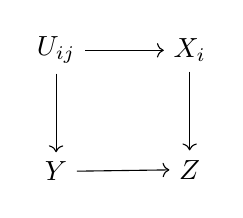
\begin{tikzpicture}
            \node (prod) {$U_{ij}$};
            \node [below = of prod] (Y) {$Y$};
            \node [right = of prod] (X) {$X_i$};
            \node [below = of X] (Z) {$Z$};
            \draw [->] (prod) -- (Y);
            \draw [->] (prod) -- (X);
            \draw [->] (X) -- (Z);
            \draw [->] (Y) -- (Z);
        \end{tikzpicture}
    \end{center}
    commutes.
    It is also not too hard to show that another scheme $W$ with compatible maps $W \to X_i \cap X_j$ and $W \to Y$ factors through $U_{ij}$.

    Hence, there is a unique isomorphism $\phi_{ij}: U_{ij} \to U_{ji}$ by the uniqueness of limits.
    Claim: The $U_i$, $U_{ij}$ and $\phi_{ij}$ satisfy the gluing conditions.
    \begin{itemize}
        \item Clearly $U_{ii} = U_i$ and so $\phi_{ii} = \mathrm{id}$ as there is a unique isomorphism $U_i \to U_i$.
        \item Note that by choice of $\phi_{ij}$ we know that the diagram
        \begin{center}
            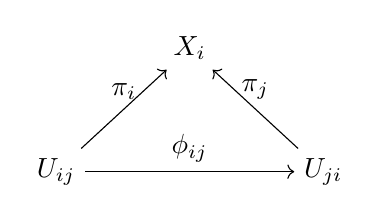
\begin{tikzpicture}
                \node (X) {$X_i$};
                \node [below left = of X] (Ui) {$U_{ij}$};
                \node [below right = of X] (Uj) {$U_{ji}$};
                \draw [->] (Ui) -- (X) node [midway, above] {$\pi_i$};
                \draw [->] (Uj) -- (X) node [midway, above] {$\pi_j$};
                \draw [->] (Ui) -- (Uj) node [midway, above] {$\phi_{ij}$};
            \end{tikzpicture}
        \end{center}
        is commutative.
        Hence $\phi_{ij}^{-1}(\pi_j^{-1}(X_i \cap X_j)) = \pi_i^{-1}(X_i \cap X_j)$ and so $\phi_{ij}^{-1}(U_{ij}) \subseteq U_{ji}$.
        \item Let
        \begin{equation*}
            U_{ijk} := \Bigl( \pi_i^{-1}(X_i \cap X_j \cap X_k), \ \restr{\O_{X}}{\pi_i^{-1}(X_i \cap X_j \cap X_k)} \Bigr) = U_{ij} \cap U_{ik}
        \end{equation*}
        A similar argument as above also shows that $U_{ijk}$ is the fiber product $(X_i \cap X_j \cap X_k) \times_Z Y$.
        Now, by uniqueness of limits, find that there is a unique isomorphism $U_{ijk} \to U_{kij}$.
        Note that both
        \begin{equation*}
            \restr{\phi_{ik}}{U_{ijk}} \quad \text{and} \quad \restr{\phi_{jk}}{U_{jik}} \circ \restr{\phi_{ij}}{U_{ijk}}
        \end{equation*}
        are such isomorphisms, hence 
        \begin{equation*}
            \restr{\phi_{ik}}{U_{ijk}} = \restr{\phi_{jk}}{U_{jik}} \circ \restr{\phi_{ij}}{U_{ijk}}
        \end{equation*}
    \end{itemize}

    \paragraph{Step 3: $Z$ affine} Exactly as in step 2 (note that we did not use $Y$ affine there).

    \paragraph{Step 4: General case} Let $Z = \bigcup Z_i$ be a cover of $Z$ by affine opens.
\end{proof}

\section{Properties of Schemes and Morphisms}

\begin{prop}
    Let $X$ be a scheme and let $P$ be a property of affine opens (i.e. a class of embeddings $\Spec R \to X$) such that
    \begin{itemize}
        \item for all $\alpha: \Spec R \to X$ and $f \in R$ have
        \begin{equation*}
           \text{$\alpha$ satisfies $P$} \quad \Rightarrow \quad \text{$\alpha_f$ satisfies $P$}
        \end{equation*}
        where $\alpha_f: \Spec R_f \to X$.
        \item for all $\alpha: \Spec R \to X$ and covers $\Spec R = \bigcup D_{f_i}$ have
        \begin{equation*}
            \text{all $\alpha_{f_i}$ satisfy $P$} \quad \Rightarrow \quad \text{$\alpha$ satisfies $P$}
        \end{equation*}
    \end{itemize}
    If there is a cover $X = \bigcup X_i$ of affine opens such that all inclusions $X_i \subseteq X$ satisfy $P$, then all inclusions $U \subseteq X$ of affine opens satisfy $P$.
\end{prop}

\begin{definition}
    A scheme $X$ is
    \begin{itemize}
        \item \emph{Noetherian}, if $|X|$ is quasi-compact and for all affine open $U$ have that $\O_X(U)$ is Noetherian.
        \item \emph{reduced}, if for all open $U$ have that $\O_X(U)$ is reduced.
        \item \emph{irreducible}, if $|X|$ is irreducible (i.e. not the union of two proper closed subsets).
        \item \emph{integral}, if for all open $U$ have that $\O_X(U)$ is integral.
    \end{itemize}
\end{definition}

\begin{definition}
    A morphism of schemes $f: X \to Y$ is
    \begin{itemize}
        \item \emph{affine}, if $f^{-1}(U)$ is affine for all affine open $U \subseteq X$.
        \item \emph{quasi-compact}, if $f^{-1}(U)$ is quasi-compact for all quasi-compact $U \subseteq X$.
        \item \emph{locally of finite type}, if for all affine opens $U \subseteq X$ and $V \subseteq Y$ with $f(U) \subseteq V$ have that $\O_X(U)$ becomes a finitely generated $\O_Y(V)$-algebra when equipped with 
        \begin{equation*}
            \O_Y(V) \ \overset{f^\#}{\to} \ \O_X(f^{-1}(V)) \ \to \ \O_X(U)
        \end{equation*}
        \item \emph{finite type}, if it is quasi-compact and locally of finite type
        \item a \emph{closed immersion}, if it is an isomorphism onto a closed subscheme of $Y$.
        \item an \emph{open immersion}, if it is an isomorphism onto an open subscheme of $Y$.
        \item \emph{flat}, if all $\O_{X, x}$ are flat $\O_{Y, f(x)}$-modules, i.e. the functor $\O_{X, x} \otimes_{\O_{Y, f(x)}} \cdot$ of $\O_{Y, f(x)}$-algebras is exact\footnote{here $\O_{X, x}$ becomes a $\O_{Y, f(x)}$-algebra via $f_x$}.
    \end{itemize}
\end{definition}

\begin{prop}
    An $R$-module $M$ is flat if and only if for all injective $\alpha: N_1 \to N_2$ have that $\mathrm{id} \otimes \alpha: M \otimes_R N_1 \to M \otimes_R N_2$ is injective.
\end{prop}

\end{document}